\documentclass[class=Poster, crop=false]{standalone}
\begin{document}
    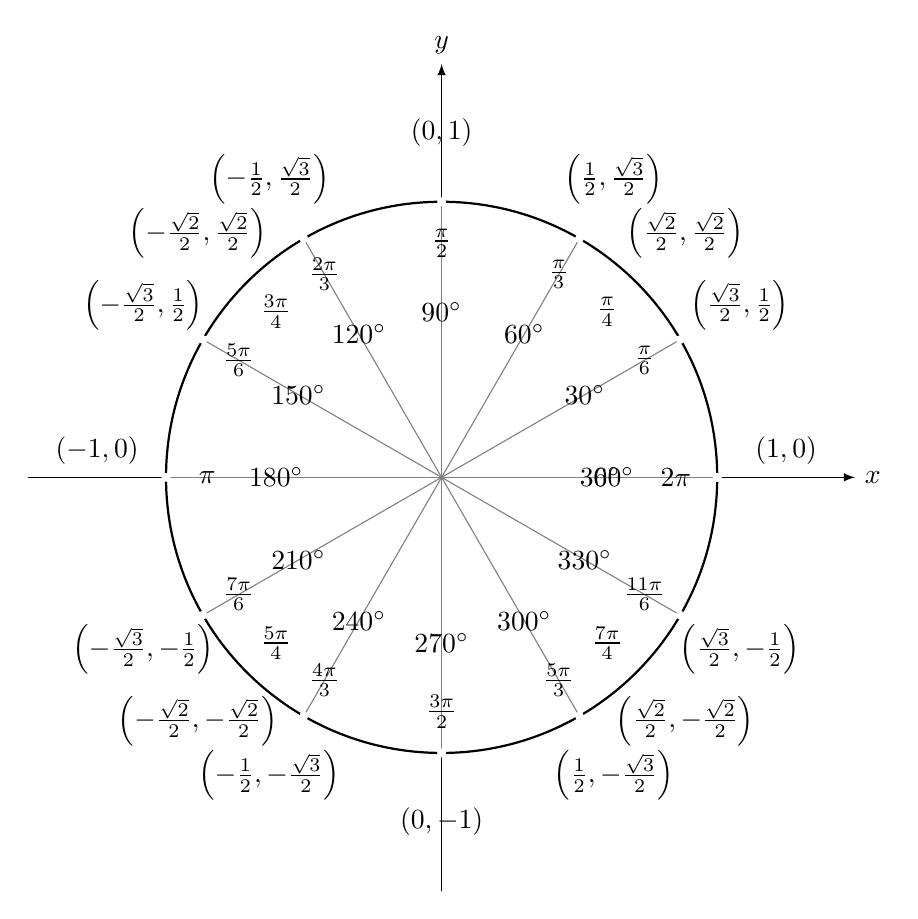
\begin{tikzpicture}[scale=3.5,cap=round,>=latex]
        % draw the coordinates
        \draw[->] (-1.5cm,0cm) -- (1.5cm,0cm) node[right] {$x$};
        \draw[->] (0cm,-1.5cm) -- (0cm,1.5cm) node[above] {$y$};

        % draw the unit circle
        \draw[thick] (0cm,0cm) circle(1cm);

        \foreach \x in {0,30,...,360} {
                % lines from center to point
                \draw[gray] (0cm,0cm) -- (\x:1cm);
                % dots at each point
                \filldraw[white] (\x:1cm) circle(0.4pt);
                % draw each angle in degrees
                \draw (\x:0.6cm) node {$\x^\circ$};
        }

        % draw each angle in radians
        \foreach \x/\xtext in {
            30/\frac{\pi}{6},
            45/\frac{\pi}{4},
            60/\frac{\pi}{3},
            90/\frac{\pi}{2},
            120/\frac{2\pi}{3},
            135/\frac{3\pi}{4},
            150/\frac{5\pi}{6},
            180/\pi,
            210/\frac{7\pi}{6},
            225/\frac{5\pi}{4},
            240/\frac{4\pi}{3},
            270/\frac{3\pi}{2},
            300/\frac{5\pi}{3},
            315/\frac{7\pi}{4},
            330/\frac{11\pi}{6},
            360/2\pi}
                \draw (\x:0.85cm) node {$\xtext$};

        \foreach \x/\xtext/\y in {
            % the coordinates for the first quadrant
            30/\frac{\sqrt{3}}{2}/\frac{1}{2},
            45/\frac{\sqrt{2}}{2}/\frac{\sqrt{2}}{2},
            60/\frac{1}{2}/\frac{\sqrt{3}}{2},
            % the coordinates for the second quadrant
            150/-\frac{\sqrt{3}}{2}/\frac{1}{2},
            135/-\frac{\sqrt{2}}{2}/\frac{\sqrt{2}}{2},
            120/-\frac{1}{2}/\frac{\sqrt{3}}{2},
            % the coordinates for the third quadrant
            210/-\frac{\sqrt{3}}{2}/-\frac{1}{2},
            225/-\frac{\sqrt{2}}{2}/-\frac{\sqrt{2}}{2},
            240/-\frac{1}{2}/-\frac{\sqrt{3}}{2},
            % the coordinates for the fourth quadrant
            330/\frac{\sqrt{3}}{2}/-\frac{1}{2},
            315/\frac{\sqrt{2}}{2}/-\frac{\sqrt{2}}{2},
            300/\frac{1}{2}/-\frac{\sqrt{3}}{2}}
                \draw (\x:1.25cm) node {$\left(\xtext,\y\right)$};

        % draw the horizontal and vertical coordinates
        % the placement is better this way
        \draw (-1.25cm,0cm) node[above=1pt] {$(-1,0)$}
              (1.25cm,0cm)  node[above=1pt] {$(1,0)$}
              (0cm,-1.25cm) node {$(0,-1)$}
              (0cm,1.25cm)  node {$(0,1)$};
    \end{tikzpicture}
\end{document}
